
\section{Wednesday for MAT3040}\index{Wednesday_lecture}
\paragraph{Reviewing}
\begin{itemize}
\item
Quotient Space:
\[
V/ W=\{\bm v+W\mid \bm v\in V\}
\]
The elements in $V/ W$ are cosets.
Note that $V/ W$ does not mean a subset of $V$.
\item
Define the canonical projection mapping
\[
\begin{array}{ll}
&\pi_W:V\to V/ W,\\
\text{with }&\bm v\mapsto \bm v+W,
\end{array}
\]
then we imply $\pi_W$ is a surjective linear transformation with $\ker(\pi_W)=W$. 

If $\dim(V)<\infty$, then by Rank-Nullity Theorem~(\ref{The:2:3}), we imply that 
\[
\dim(V)=\dim(W) + \dim(V/ W),
\]
i.e., $\dim(V/ W) = \dim(V) - \dim(W).$
\item
\textbf{(Universal Property I)} Every linear transformation $T:V\to W$ with $V'\le\ker(T)$ can be descended to the composition of the canonical projection mapping $\pi_{V'}$ and the mapping
\[
\begin{array}{ll}
&\tilde{T}:V/ V'\to W\\
\text{with }&\bm v+V'\mapsto T(\bm v).
\end{array}
\]
In other words, the diagram (2.1) commutes:
\begin{figure}[H]
\centering
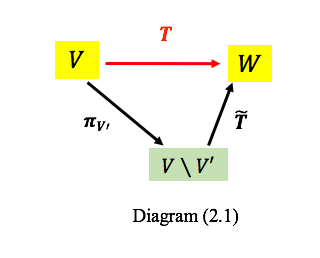
\includegraphics[width=0.4\textwidth]{week4/p_2}
\end{figure}
In other words, the mapping starting from either the black or red line gives the same result, i.e., $T(\bm v) = \tilde{T}\circ \pi_{V'}(\bm v) = \tilde{T}(\bm v+V')$ for any $\bm v\in V$. 
\item
\textbf{(First Isomorphism Theorem)}
Under the setting of Universal Property I~(UPI), if $T$ is a surjective linear transformation with $V'=\ker(T)$, then the $\tilde{T}$ is an isomorphism.
\end{itemize}

\begin{example}
Suppose that $U,W\le V$ with $U\cap W = \{\bm0\}$, then define the mapping
\[
\begin{array}{ll}
&\phi:U\oplus W\to U\\
\text{with }&\phi(\bm u+\bm w) = \bm u
\end{array}
\]
\begin{remark}
Exercise: if $U,W\le V$ but $U\cap W\ne\{\bm0\}$, then the mapping
\[
\begin{array}{ll}
&\phi:U+ W\to U\\
\text{with }&\bm u+\bm w \mapsto \bm u
\end{array}\qquad
\text{is not well-defined:}
\]
Suppose that $\bm0\ne\bm v\in U\cap W$ and for any $\bm u\in U,\bm w\in W$, we construct 
\[
\begin{array}{ll}
\bm u'=\bm u-\bm v\in U,
&
\bm w'=\bm w+\bm v\in V
\end{array}\implies
\phi(\bm u'+\bm w')=\bm u-\bm v
\]
Therefore we get $\bm u+\bm w=\bm u'+\bm w'$ but $\phi(\bm u+\bm w)\ne\phi(\bm u'+\bm w')$.
\end{remark}

Back to the situation $U\cap W=\{\bm0\}$, then it's clear that 
$\phi:U\oplus W\to U$ is surjective linear transformation with $\ker(\phi)=W$. 
Therefore, construct the new mapping
\[
\begin{array}{ll}
&\tilde{\phi}:U\oplus W/ W\to U\\
\text{with }&\bm u+\bm w+W\mapsto\phi(\bm u+\bm w)
\end{array}
\]
We imply $\tilde{\phi}$ is an isomorphism by First Isomorphism Theorem.
\end{example}

Now we study the generalized quotients, which is defined to satisfy the generalized version of universal property I.

\begin{definition}[Universal Property for Quotients]
Let $V$ be a vector space and $V'\le V$. Consider the collection of linear transformations
\[
\text{Obj}=\left\{T:V\to W\middle| 
\begin{aligned}
&\text{$T$ is a linear transformation}\\
&V'\le\ker(T)
\end{aligned}
\right\}
\]
(For example, $\pi_{V'}:V\to V/ V'$ is an element from the set $\text{Obj}$.)

An element $(\phi: V\to U)\in\text{Obj}$ is said to satisfy the \emph{universal property} if it satisfies the following:
\begin{quotation}
Given any element $(T:V\to W)\in\text{Obj}$, 
we can extend the transformation $\phi$ with a \emph{uniquely existing} $\tilde{T}:U\to W$ so that the diagram~(2.2) commutes:
\begin{figure}[H]
\centering
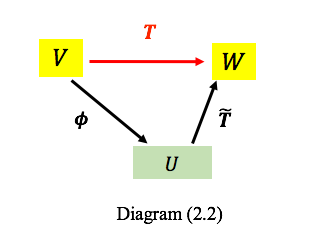
\includegraphics[width=0.4\textwidth]{week4/p_3}
\end{figure}
Or equivalently, for given $(T:V\to W)\in\text{Obj}$, there exists the \emph{unique} mapping $\tilde{T}:U\to W$ such that $T=\tilde{T}\circ\phi$.
\end{quotation}
\end{definition}

\begin{theorem}[Universal Property II]
\begin{enumerate}
\item
The mapping $(\pi_{V'}: V\to V/ V')\in\text{Obj}$ is a universal object, i.e., it satisfies the universal property.
\item
If $(\phi:V\to U)$ is a universal object, then $U\cong V/ V'$, i.e., 
there is intrinsically ``one'' element in the set of universal objects.
\end{enumerate}
\end{theorem}
\begin{proof}
\begin{enumerate}
\item
Consider any linear transformation $T:V\to W$ such that $V'\le\ker(T)$, 
then define (construct) the same $\tilde{T}:V/ V'\to W$ as that in UPI. 
Therefore, for given $T$, applying the result of UPI, we imply $T=\tilde{T}\circ\pi_{V'}$, i.e., $\pi_{V'}$ satisfies the diagram~(2.2).

To show the uniqueness of $\tilde{T}$, suppose there exists $\tilde{S}:V/ V'\to W$ such that the diagram~(2.3) commutes.
\begin{figure}[H]
\centering
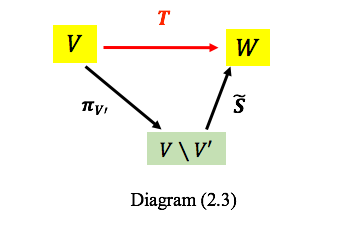
\includegraphics[width=0.4\textwidth]{week4/p_4}
\end{figure}
It suffices to show the mapping $\tilde{S}=\tilde{T}$: for any $\bm v+V'\in V/ V'$, we have
\[
\tilde{S}(\bm v+V'):=\tilde{S}\circ\pi_{V'}(\bm v)=T(\bm v),
\]
where the first equality is due to the surjectivity of $\pi_{V'}$.
By the result of UPI, $T(\bm v)=\tilde{T}(\bm v+V')$. Therefore $\tilde{T}(\bm v+V') = \tilde{S}(\bm v+V')$ for all $\bm v+V'\in V/ V'$. The proof is complete.
\item
Suppose that $(\phi:V\to U)$ satisfies the universal property. In particular, the following two diagrams hold:
\begin{figure}[H]
\centering
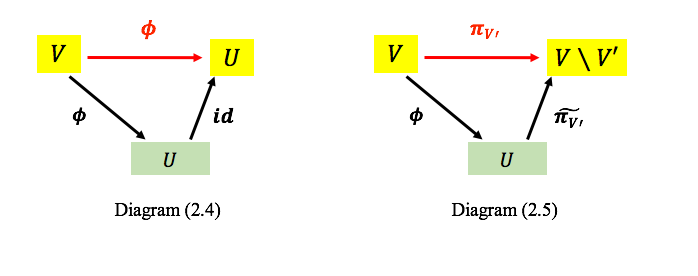
\includegraphics[width=0.7\textwidth]{week4/p_5}
\end{figure}
Since $(\pi_{V'})$ satisfies the universal property, in particular, the following two diagrams hold:
\begin{figure}[H]
\centering
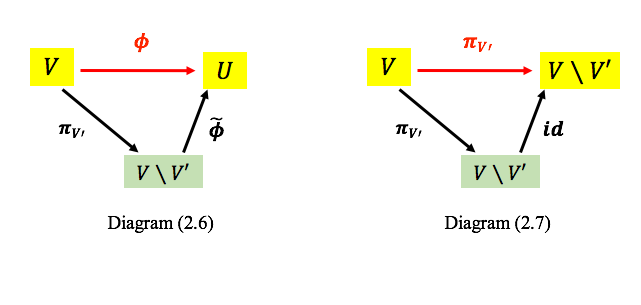
\includegraphics[width=0.7\textwidth]{week4/p_6}
\end{figure}

Then we claim that: Combining Diagram~(2.5) and (2.6), we imply the diagram~(2.8):
\begin{figure}[H]
\centering
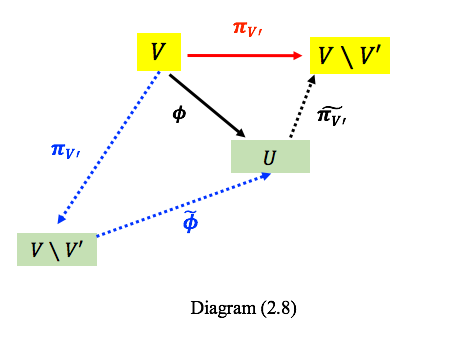
\includegraphics[width=0.7\textwidth]{week4/p_7}
\caption*{Graph Description: Note that this diagram commutes, i.e., the mapping starting from either the red line or the dash line gives the same result, i.e., $\pi_{V'} = \tilde{\pi}_{V'}\circ\tilde{\phi}\circ\pi_{V'}$.
Comparing Diagram~(2.7) and Diagram~(2.8), we have $\tilde{\pi}_{V'}\circ\tilde{\phi}=id$, by the 
\emph{uniqueness} of the universal object.
}
\end{figure}
Therefore, $\tilde{\pi}_{V'}\circ\tilde{\phi}=id$ implies $\tilde{\pi}_{V'}$ is surjective and $\tilde{\phi}$ is injective.

Also, combining Diagram~(2.6) and (2.5), we imply diagram~(2.9):
\begin{figure}[H]
\centering
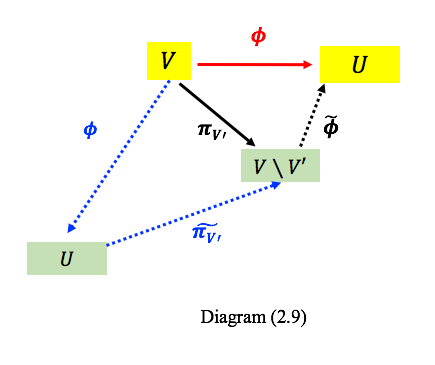
\includegraphics[width=0.7\textwidth]{week4/p_8}
\caption*{Graph Description: Note that this diagram commutes, i.e., the mapping starting from either the red line or the dash line gives the same result, i.e., $\phi = \tilde{\phi}\circ\tilde{\pi}_{V'}\circ\phi$.
Comparing Diagram~(2.9) and Diagram~(2.4), we have $\tilde{\phi}\circ\tilde{\pi}_{V'}=id$,
by the \emph{uniqueness} of the universal object
}
\end{figure}
Therefore, $\tilde{\phi}\circ\tilde{\pi}_{V'}=id$ implies $\tilde{\phi}$ is surjective and $\tilde{\pi}_{V'}$ is injective.

Therefore, both $\tilde{\phi}:U\to V/ V'$ and $\tilde{\pi}_{V'}:V/ V'\to U$ are bijective, i.e., $U\cong V/ V'$. The proof is complete.
\end{enumerate}
\end{proof}

\subsection{Dual Space}
\begin{definition}
Let $V$ be a vector space over a field $\mathbb{F}$. The \emph{dual vector space} $V^*$ is defined as
\begin{align*}
V^*&=\text{Hom}_{\mathbb{F}}(V,\mathbb{F})\\
&=\{f:V\to\mathbb{F}\mid \text{$f$ is a linear transformation}\}
\end{align*}
\end{definition}

\begin{example}
\begin{enumerate}
\item
Consider $V=\mathbb{R}^n$ and define $\phi_i:V\to\mathbb{R}$ as the $i$-th component of input:
\[
\phi_i\begin{pmatrix}
x_1\\\vdots\\x_n
\end{pmatrix}=x_i,
\]
Then we imply $\phi_i\in V^*$.  On the contrary, $\phi_i^2\begin{pmatrix}
x_1\\\vdots\\x_n
\end{pmatrix}=x_i^2$ is not in $V^*$
\item
Consider $V=\mathbb{F}[x]$ and define $\phi:V\to\mathbb{F}$ as:
\[
\phi(p(x))=p(1),
\]
It's clear that $\phi\in V^*$:
\begin{align*}
\phi(ap(x)+bq(x))&=ap(1)+bq(1)\\
&=a\phi(p(x))+b\phi(q(x))
\end{align*}
\item
Also, $\psi:V\to\mathbb{F}$ by $\psi(p(x))=\int_0^1p(x)\diff x$ is in $V^*$.
\item
Also, for $V=M_{n\times n}(\mathbb{F})$, the mapping $\text{tr}:V\to\mathbb{F}$ by $\text{tr}(M)=\sum_{i=1}^nM_{ii}$ is in $V^*$. However, the $\text{det}:V\to\mathbb{F}$ is not in $V^*$
\end{enumerate}
\end{example}


\begin{definition}
Let $V$ be a vector space, with basis $B=\{v_i\mid i\in I\}$ 
($I$ can be finite or countable, or uncountable). 
Define
\[
B^*=\{f_i:V\to\mathbb{F}\mid i\in I\},
\]
where $f_i$'s are defined on the basis $B$:
\[
f_i(v_j)=\delta_{ij}=\left\{
\begin{aligned}
1,&\quad \text{if }i=j\\
0,&\quad \text{if }i\ne j
\end{aligned}
\right.
\]
Then we extend $f_i$'s linearly, i.e., for $\sum_{j=1}^N\alpha_jv_j\in V$,
\[
f_i(\sum_{j=1}^N\alpha_jv_j)=\sum_{i=1}^N\alpha_jf_i(v_j).
\]
It's clear that $f_i\in V^*$ is well-defined. 
\end{definition}
Our question is that whether the $B^*$ can be the basis of $V^*$?






















